\documentclass{article}
\usepackage[a4paper,margin=1in]{geometry}

\usepackage{graphicx}
\usepackage{times}
\usepackage{float}
\usepackage{booktabs}
\usepackage{amsmath,amssymb,amsthm}
\usepackage{url}
\usepackage[hidelinks]{hyperref}
\usepackage{caption}

\captionsetup{font=small,labelfont=bf}
\newtheorem{problem}{Problem}

\title{Two-Tier Reinforcement Learning with an Oracle-Free\\
Top-$K$ Search for Deep Learning Job Scheduling\\
on Heterogeneous GPU Clusters}

\author{Ali Ahmadi Esfidi\\ \small Department of Mathematics and Computer Science, Amirkabir University of Technology\\ \small \texttt{ali.ahmadi2004@aut.ac.ir}}
\date{\today}

\begin{document}
\maketitle

\begin{abstract}
Efficient job scheduling is crucial for maximizing the utilization of
heterogeneous GPU clusters that run machine learning workloads. Traditional
heuristic- or optimization-based methods often fail to adapt when job types or
hardware availability change. We present a two-tier reinforcement learning
scheduler: an inner agent assigns jobs to accelerators and an outer agent decides
whether to duplicate a job onto additional hardware. On the Gavel throughput
dataset the complete two-tier system reaches a mean cumulative throughput of
$17.91$, above the inner agent alone ($15.15$), a total-throughput greedy oracle
($16.10$), and Sia ($14.85$), a state-of-the-art goodput-optimized cluster
scheduler---while consuming only observable state at decision time.

Analysing where the inner agent loses to the oracle shows that the deficit is one
of \emph{selection among near-ties}: re-scoring just the $K$ most probable actions
with the true reward already exceeds the full-space oracle ($17.21$ at $K{=}5$).
That refinement is not deployable, however, because scoring a candidate requires
the co-location throughput of a placement that has not been made. The second half
of this paper removes that dependency. We show the reward of a placement is
determined by an $18$-dimensional sufficient statistic readable from the
scheduler's own bookkeeping; slots sharing it are provably reward-equivalent, so a
small weight-shared network over it predicts the oracle's quantity with
$R^2 = 0.99972$. The resulting oracle-free search reproduces the oracle-assisted
one on the held-out test sets ($17.48$ against $17.21$), beats the greedy oracle
by $+1.38$ (paired $t = 4.70$), and composes with the duplication tier to give the
strongest configuration we measure, $19.76$ against $17.91$ for the two-tier
system alone. Bootstrapped online from realised rewards alone---one label per
decision, no prior profiling---it recovers that performance after about $1{,}500$
labels.

We report negative results in the same detail. Learned long-horizon value and
$Q$-heads are dominated by their own estimation error and lose to the myopic
score; continual online policy updates cost more in exploration than they return
within the horizon tested; and a model that never saw two of the five job families
is badly wrong on them ($63\times$ the prediction error) yet barely loses end-to-end
throughput, because the policy's candidate set bounds the cost of mispricing.
Training uses randomly generated job sets throughout; the $20$ held-out sets are
used only to report, and configurations are selected on a separate validation
stream.
\end{abstract}


\section{Introduction}
Efficient job scheduling is an important challenge in modern computing systems. The rapid increase of machine learning workloads has created a strong need for effective use of heterogeneous hardware resources, especially GPUs. Traditional scheduling methods often rely on heuristics or fixed optimization strategies. While these methods are simple, they do not adapt well to dynamic environments where job requirements and resource availability change over time. As a result, they cannot fully take advantage of the performance potential of large computing clusters \cite{luo2025prediction}.

Distributed deep learning (DDL) is powering leaps in NLP, computer vision, and networking. That said, the training process for deep neural networks consumes enormous computational horsepower—most organizations must turn to dedicated GPU clusters \cite{weng2022mlaas}.

Scheduling in deep learning training is inherently a sequential decision problem, where each action influences future resource availability. Locality sensitivity and dynamic fragmentation further complicate the process, limiting the effectiveness of heuristic-based approaches \cite{luan2019sched2}.

New generations of GPUs support Multi-Instance GPU (MIG), which partitions a physical GPU into several isolated instances. 
This enables multiple workloads or multiple users to run workloads simultaneously on one GPU, maximizing utilization while ensuring performance isolation and guaranteed quality of service (QoS) \cite{nvidiaMIG}.
In the context of heterogeneous cluster scheduling, MIG effectively transforms one accelerator into multiple ``virtual GPUs,'' supporting finer-grained allocation and improving overall system efficiency.
With the rapid growth of DDL workloads, understanding the behavior of such jobs in real-world GPU clusters has become increasingly important.  Traditional heuristic schedulers often fail to capture the highly dynamic characteristics of these workloads.  Key challenges include:
\begin{itemize}
  \item \textbf{GPU Heterogeneity}: Modern clusters contain multiple GPU architectures (e.g., V100, A100, H100), each with different performance characteristics.  An effective scheduler must account for these differences to maximize cluster utilization.
  \item \textbf{Space Sharing on a Single GPU}: Technologies such as NVIDIA MIG allow a single physical GPU to be partitioned into several isolated “virtual GPUs,” enabling multiple workloads or users to run simultaneously while preserving performance isolation.
  \item \textbf{Distributed Deep Learning Across Multiple GPUs}: Training a single deep-learning job typically requires data or model parallelism across many GPUs.  Schedulers must co-locate these GPUs to reduce communication overhead and maintain high throughput.
  \item \textbf{Unknown or Variable Throughput per Workload}: The actual performance of a workload on each GPU type is often unknown in advance and can vary over time, making accurate prediction and adaptive scheduling essential.
  \item \textbf{Sequential and Dynamic Decision Process}: Job arrivals and completions occur continuously, so every scheduling action affects future resource availability.  The scheduler must make fast, online decisions in a constantly changing environment.
  \item \textbf{Combinatorial Complexity and NP-Hardness}: The assignment space of jobs to heterogeneous GPUs grows combinatorially with cluster size, and the objective function is non-separable, placing the scheduling problem firmly in the class of NP-hard problems.
\end{itemize}

Reinforcement learning (RL) offers a promising direction for this problem. Instead of following predefined rules, RL agents can learn adaptive strategies directly from experience. By observing the system state and receiving feedback from past decisions, an RL-based scheduler can improve over time. Prior work has demonstrated that RL is a powerful framework for tackling this challenge, showing it can significantly increase hardware utilization, reduce job completion times, and improve overall throughput~\cite{luan2019sched2,mao2019learning,venkataswamy2022launchpad}.


In this paper, we introduce a dual-agent RL method for job scheduling in heterogeneous GPU clusters. The method is built around two agents that work together. The inner agent assigns jobs to specific GPUs based on workload performance profiles. The outer agent decides whether to duplicate jobs in order to improve overall throughput. This hierarchical structure allows the system to combine local scheduling efficiency with global optimization.

We evaluate our method using the \texttt{Gavel} throughput dataset, which provides performance measurements for deep learning workloads on heterogeneous GPU architectures. Both agents are trained with Proximal Policy Optimization (PPO)~\cite{schulman2017ppo}, and we compare the learned schedulers against random placement, two greedy policies derived from Gavel, and Sia~\cite{zhong2023sia}, a state-of-the-art heterogeneity-aware, goodput-optimized cluster scheduler.

Finally, we design a joint training phase where both agents are trained at the same time. The inner agent begins from its best pre-trained model, and both agents then refine their policies together. This joint training speeds up convergence and leads to higher cumulative throughput. The results demonstrate that coordinated multi-agent learning is an effective strategy for job scheduling in heterogeneous computing environments.





The second contribution of this paper follows from a diagnosis of the first.
Section~\ref{sec:inner-results} shows that the inner agent's remaining gap to the
max-total oracle is not a gap in information but in \emph{tie-breaking}: because
throughput depends only on the accelerator type and the co-located job, many slots
have identical value, and a single arg\,max is an arbitrary choice among
near-optimal placements. Re-scoring only the top-$K$ actions the policy proposes,
and keeping the best, already surpasses the oracle. But that refinement scores
candidates with the true reward---the exact co-location throughput of a placement
that has not happened---so it is an offline upper bound, not a scheduler. We
therefore ask whether the search survives the removal of the oracle, and show that
it does, at no measurable cost in quality.

\paragraph{Contributions.}
\begin{enumerate}\itemsep2pt
\item \textbf{A two-tier RL scheduler} that separates placement from
  duplication and surpasses both a greedy throughput oracle and Sia while acting
  from observable state alone (Sections~\ref{sec:method}--\ref{sec:outer}).
\item \textbf{An exact, observable sufficient statistic for the placement reward}
  (Section~\ref{sec:canon}), which collapses reward-equivalent slots and reduces
  the learning problem to a small shared function. Its exactness is verified
  against the environment rather than assumed.
\item \textbf{An oracle-free top-$K$ search} (Section~\ref{sec:search}) that
  reproduces the oracle-assisted refinement on the held-out test sets, composes
  with the duplication tier, and can be bootstrapped online from realised rewards
  with no prior cluster profiling (Section~\ref{sec:online-reward}).
\item \textbf{A clean train/select/test separation} (Section~\ref{sec:protocol}):
  training on randomly generated job sets, configuration selection on a disjoint
  validation stream, and reporting on the held-out sets alone---together with the
  negative results this discipline exposes.
\end{enumerate}

The remainder of the paper is organised as follows.
Section~\ref{sec:method} presents the two-tier scheduler and its two agents;
Section~\ref{sec:oraclefree} develops the oracle-free search, from the sufficient
statistic through the learned components to the online variants;
Section~\ref{sec:protocol} states the train/select/test separation we hold to
throughout; and Section~\ref{sec:results} reports the results, including the two
components that did not work.

\section{Related Work}
\label{sec:related}

Efficient job scheduling and resource management in heterogeneous GPU clusters
has recently received significant attention.

Luo et al.~\cite{luo2025prediction} propose \emph{A-SRPT}, an adaptive
shortest-remaining-processing-time-first scheduler for distributed deep
learning with mixed parallelisms on GPU clusters.  By modeling each job as a
communication graph and using a random-forest regressor to predict training
iterations, A-SRPT combines a heavy-edge GPU-mapping heuristic with a
prediction-assisted SRPT framework to minimize inter-server traffic and total
job completion time, achieving up to a 92\% reduction in flow time over
state-of-the-art baselines.

Debner et al.~\cite{pmlr-v233-debner24a} demonstrate that deep reinforcement
learning (DRL) can schedule conditional task graphs in heterogeneous settings.
Selvan et al.~\cite{selvan2024pepr} introduce the \emph{PePR} metric, which
evaluates deep learning models based on performance per resource unit, showing
that smaller models can outperform large-scale ones in resource-constrained
environments.

Efficient resource management in clusters is also explored by
Chen et al.~\cite{chen2023two}, who employ a two-tiered optimization framework
with DRL to handle capacity guarantees and failures.  Building on similar
ideas, the GOGH method leverages correlation-based neural estimation and RL to
achieve adaptive throughput prediction and enhanced performance in heterogeneous
GPU clusters.

Venkataswamy et al.~\cite{venkataswamy2022launchpad} show that pre-training RL
agents with offline data from heuristic or oracle policies—as in their
\emph{Launchpad} method—enhances convergence speed and efficiency in job
scheduling for green datacenters, providing a foundation for our
approach’s dual-agent design.

Gao et al.~\cite{gao2022deep} present \emph{Aryl}, a cluster scheduler designed
to manage training and inference workloads in GPU clusters.  Aryl introduces
capacity loaning and elastic scaling to improve GPU utilization and reduce job
queuing times, employing heuristics to minimize preemptions and optimize job
completion times.

Finally, He et al.~\cite{he2025cuasmrl} propose \emph{CuAsmRL}, which utilizes
DRL to enhance SASS schedules, achieving up to a 26\% performance gain.  This
work further motivates our two-tier RL approach for scheduling in heterogeneous
GPU clusters.

Closest to our evaluation setting, Jayaram Subramanya
et al.~\cite{zhong2023sia} propose \emph{Sia}, a heterogeneity-aware cluster
scheduler that jointly chooses each job's GPU type and GPU count.  Sia builds a
goodput matrix over all (job, configuration) pairs, row-normalizes it so that
utilities become comparable across jobs, and solves a single integer linear
program per scheduling round under cluster-capacity constraints, with a
fairness exponent that trades throughput against equal progress.  We use Sia as
our principal heuristic baseline because it is the strongest published method
that reasons about GPU heterogeneity and multi-GPU allocation in the same
optimization.

Collectively, these studies motivate our formulation of job scheduling as a
reinforcement learning problem, in which we train PPO agents on the Gavel
dataset and compare them against greedy oracles and Sia.

\section{Problem Formulation}
To formally define the job scheduling problem with duplication, let $\mathcal{S}$ denote the set of servers, and let $\mathcal{A}$ be the set of accelerator types (e.g., different GPU models). Let $\mathcal{J}$ represent the set of jobs active in the cluster, and define $\mathcal{C}$ as the set of valid job combinations. Since we allow at most two jobs to share an accelerator, each combination $c \in \mathcal{C}$ contains either one or two jobs. Let $m_j(c) \in \{0,1,2\}$ denote the number of times job $j \in \mathcal{J}$ appears in combination $c$.

The throughput of job $j$ on accelerator type $a \in \mathcal{A}$ under combination $c$ is denoted by $T_{a,j}^c \geq 0$. This value is measured or estimated from profiling and reflects the performance of $j$ when co-executed with the other jobs in $c$.  

We introduce binary decision variables $x_{a,s}^c \in \{0,1\}$, where $x_{a,s}^c = 1$ indicates that combination $c$ is assigned to an accelerator of type $a$ on server $s \in \mathcal{S}$, and $x_{a,s}^c = 0$ otherwise.

The goal is to maximize the overall throughput while allowing limited job duplication. Each job must be scheduled at least once and at most twice, ensuring that duplication is possible but bounded.  

\begin{table}[t]
    \centering
    \caption{Important Notations.}
    \label{tab:notation}
    \fontsize{8}{9}\selectfont
    \begin{tabular}{|c|p{5.5cm}|} \hline
        \textbf{Symbol} & \textbf{Definition} \\ \hline\hline
        $\mathcal{S}$ & Set of all servers \\ \hline
        $\mathcal{A}$ & Set of all accelerator types \\ \hline
        $\mathcal{J}$ & Set of all jobs \\ \hline
        $\mathcal{C}$ & Set of job combinations \\ \hline
        $\mathcal{C}_{j}$ & Set of job combinations containing job $j$ \\ \hline
        $\vert c\vert$ & Number of jobs in combination $c\in\mathcal{C}$ \\ \hline
        $m_j(c)$ & Multiplicity of job $j$ in combination $c$, $m_j(c)\in\{0,1,2\}$ \\ \hline
        $T_{a,j}^{c}$ & Throughput of job $j$ on accelerator of type $a$ when combination $c$ is assigned \\ \hline
        $x_{a,s}^{c}$ & Placement of combination $c$ on accelerator of type $a$ in server $s$ \\ \hline
    \end{tabular}
\end{table}

\begin{problem}[GPU allocation problem]\label{prob:dup_milp}
\fontsize{8}{9}\selectfont
\begin{subequations}
\begin{align}
\max_{x_{a,s}^c} \quad & 
\sum_{s \in \mathcal{S}} \sum_{a \in \mathcal{A}} \sum_{c \in \mathcal{C}} \sum_{j \in \mathcal{J}}
m_j(c) \, T_{a,j}^c \, x_{a,s}^c  \label{eq:obj} \\[6pt]
\text{s.t.} \quad 
& \sum_{c \in \mathcal{C}} x_{a,s}^c \le 1, 
&& \forall s \in \mathcal{S}, \ \forall a \in \mathcal{A}, \label{eq:c1} \\[6pt]
& 1 \le \sum_{s \in \mathcal{S}} \sum_{a \in \mathcal{A}} \sum_{c \in \mathcal{C}}
m_j(c) \, x_{a,s}^c \le 2, 
&& \forall j \in \mathcal{J}, \label{eq:c2} \\[6pt]
& x_{a,s}^c \in \{0,1\}, 
&& \forall c \in \mathcal{C}, \ \forall s \in \mathcal{S}, \ \forall a \in \mathcal{A}. \label{eq:c3}
\end{align}
\end{subequations}
\end{problem}


\noindent
The formulation can be summarized as follows:
\begin{itemize}
    \item \textbf{Objective (\ref{eq:obj}):} Maximize the total throughput across all accelerators by selecting the best set of job combinations.
    \item \textbf{Constraint (\ref{eq:c1}):} Each accelerator can host at most one combination of jobs.
    \item \textbf{Constraint (\ref{eq:c2}):} Each job must be assigned at least once and at most twice, enabling controlled duplication.
    \item \textbf{Constraint (\ref{eq:c3}):} Decision variables are binary.
\end{itemize}

\begin{figure*}[!t]
    \centering
    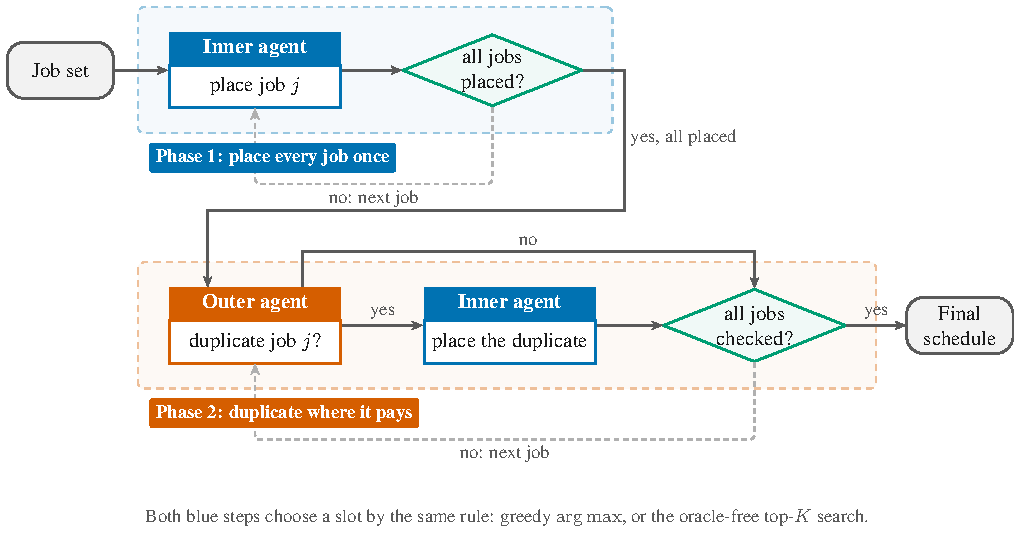
\includegraphics[width=\textwidth]{images/workflow.pdf}
    \caption{The two-tier workflow. In phase~1 the inner agent places every queued job
exactly once. In phase~2 the outer agent walks the resulting schedule and decides,
per job, whether to duplicate it; each duplicate is returned to the inner tier for
placement. Both tiers choose a slot by the same rule---the greedy $\arg\max$ of
Section~\ref{sec:method}, or the oracle-free top-$K$ search of
Section~\ref{sec:oraclefree}, which is a drop-in replacement for it.}
    \label{fig:dig}
\end{figure*}
\subsection{Computational Complexity of the Assignment Problem}
\label{subsec:complexity}

The core assignment problem, even without considering job duplication, is computationally intractable. To understand its complexity, consider a cluster with:
\begin{itemize}
    \item $\mathcal{J}$: a set of $J$ jobs to assign,
    \item $\mathcal{S}$: a set of $S$ servers,
    \item $\mathcal{A}$: a set of $A$ accelerator types \textit{per server} (e.g., K80, P100, V100).
\end{itemize}
This defines $S \times A$ total GPU ``slots.'' While assigning one job per GPU is a standard matching problem, the complexity explodes due to two critical factors:

\textbf{(a) Co-location of Jobs:}
The fundamental unit of assignment is not a single job but a \textit{job combination} $c \in \mathcal{C}$, where a combination can be a single job or a pair of jobs. The size of the set $\mathcal{C}$ grows combinatorially with the number of jobs:
\begin{itemize}
    \item Number of single-job combinations: $J$
    \item Number of two-job combinations: $\binom{J}{2} = \frac{J(J-1)}{2}$
    \item Total possible combinations: $|\mathcal{C}| = J + \frac{J(J-1)}{2} = {O(J^2)}$
\end{itemize}
The scheduler must choose which of these $O(J^2)$ combinations to place on each of the $S \times A$ GPUs.

\textbf{(b) Performance Heterogeneity:}
The throughput $T^{c}_{a,j}$ of a job $j$ is not a constant value but depends on:
\begin{itemize}
    \item The \textit{GPU type} $a$ (e.g., a job runs faster on a V100 than on a K80).
    \item The \textit{job combination} $c$ (i.e., the other job it is co-located with, if any). The performance interference between two jobs is unique to each pair and each GPU type.
\end{itemize}
\
\subsection{Generalized Scheduling Problem (no duplication, per–job variables)}

We eliminate the combination index and introduce binary decision variables
\[
x_{a,s}^{j} =
\begin{cases}
1 & \text{if job $j$ is assigned to accelerator type $a$ on server $s$},\\
0 & \text{otherwise.}
\end{cases}
\]

\begin{align}
\max\ Z \;=\;&
\underbrace{\sum_{s\in\mathcal{S}}\sum_{a\in\mathcal{A}}\sum_{j\in\mathcal{J}}
T_{a,j}\,x_{a,s}^{j}}_{\text{total throughput}}
\;+\;
\underbrace{\sum_{s\in\mathcal{S}}\sum_{a\in\mathcal{A}}
\sum_{\substack{j<k\\ j,k\in\mathcal{J}}}
Q_{a,s}(j,k)\,x_{a,s}^{j} x_{a,s}^{k}}_{\text{pairwise synergy/penalty}}
\label{eq:obj_job}
\end{align}

subject to
\begin{align}
& \sum_{j\in\mathcal{J}} x_{a,s}^{j} \le 2
&& \forall s\in\mathcal{S},\ \forall a\in\mathcal{A}
\label{eq:one_per_accel}\\[4pt]
& \sum_{s\in\mathcal{S}}\sum_{a\in\mathcal{A}} x_{a,s}^{j} = 1
&& \forall j\in\mathcal{J}
\label{eq:each_job_once}\\[4pt]
& x_{a,s}^{j} \in \{0,1\}
&& \forall j\in\mathcal{J},\ \forall s\in\mathcal{S},\ \forall a\in\mathcal{A}.
\label{eq:binary}
\end{align}

\paragraph{Explanation}
\begin{itemize}
  \item \eqref{eq:obj_job}: maximize total throughput plus any pairwise interaction bonuses/penalties \(Q_{a,s}(j,k)\).
  \item \eqref{eq:one_per_accel}: each accelerator can host at most two jobs.
  \item \eqref{eq:each_job_once}: each job is assigned \emph{exactly once}.
  \item \eqref{eq:binary}: decision variables are binary.
\end{itemize}

This yields a mixed-integer quadratic program (MIQP) equivalent to the earlier formulation but with
\(|\mathcal{J}|\,|\mathcal{A}|\,|\mathcal{S}|\) binary decision variables.


Consequently, the ``best'' placement for a job cannot be pre-computed in isolation;
it depends on its co-location partner and the specific hardware,
making the problem inherently non-linear and non-separable.
The assignment space grows combinatorially---\(O(J^{2})\) even before
considering hardware types---and the quadratic objective with pairwise
interaction terms renders the problem strongly NP-hard.
These factors motivate the use of approximate methods,
such as reinforcement learning, to obtain near-optimal solutions efficiently.


\subsection{Justification for Reinforcement Learning}
\label{sec:justification}

The problem of job scheduling on heterogeneous GPUs is a combinatorial optimization problem proven to be NP-Hard. While solvers can find near-optimal solutions for small, offline instances, they are unsuitable for large-scale, online cluster environments due to computational intractability, the sequential and uncertain nature of job arrivals, and dynamic system conditions~\cite{mao2019learning, weng2022mlaas}.

We employ a Reinforcement Learning (RL) framework because it directly addresses these challenges:
\begin{itemize}
   \item \textbf{Scalability:} Once trained, an RL policy makes fast scheduling decisions via a forward pass through a neural network, bypassing the need for expensive online computation~\cite{mao2019learning}.
    \item \textbf{Online Sequential Decision-Making:} RL is inherently designed for making decisions under uncertainty without prior knowledge of the future job queue, optimizing for long-term cumulative reward~\cite{sutton2018reinforcement}.
    \item \textbf{Robustness to Dynamics:} RL agents learn from experience in a simulated environment, crafting policies that are robust to noise, performance variability~\cite{wang2018perturbed}, and changes in cluster state.
    \item \textbf{Generalization:} A trained agent can generalize its policy to new, unseen job mixes and cluster configurations, unlike solvers which must start from scratch for every new scenario \cite{mao2018decima}.
\end{itemize}
Therefore, RL provides a powerful framework for learning a fast, adaptive, and high-performance scheduling policy for real-world deployment.

\subsection{NP-Hardness of the GPU Allocation Problem}

We consider the following formal GPU allocation problem:
\begin{align}
    \max \quad & \sum_{s \in S} \sum_{a \in A} \sum_{c \in C} \sum_{j \in J} m_j(c) T^c_{a,j} x^c_{a,s} \\
    \text{s.t.} \quad & \sum_{c \in C} x^c_{a,s} \leq 1 \quad \forall s \in S, a \in A \\
    & 1 \leq \sum_{s \in S} \sum_{a \in A} \sum_{c \in C} m_j(c) x^c_{a,s} \leq 2 \quad \forall j \in J \\
    & x^c_{a,s} \in \{0,1\} \quad \forall c \in C, a \in A, s \in S
\end{align}

\subsubsection*{Step 1: Problem Simplification}
Ignoring duplication and interaction effects (i.e., letting $m_j(c)=1$ and each job assigned exactly once), the problem reduces to assigning jobs to GPUs such that each GPU hosts at most $k$ jobs with additive throughput. This is the well-studied Generalized Assignment Problem (GAP), known to be strongly NP-hard \cite{ShmoysTardos1993}.

\subsubsection*{Step 2: Incorporating Interaction and Duplication}
When the interaction term $m_j(c)$ and duplication constraints are included:
\begin{itemize}
    \item Throughput is non-additive and depends on both job combinations and GPU type.
    \item Each job can be scheduled once or duplicated, increasing assignment possibilities.
\end{itemize}
This results in a problem strictly harder than GAP, as the profit from assigning jobs depends on subsets of jobs on each GPU.

\subsubsection*{Step 3: Proof Sketch}
\begin{enumerate}
    \item Map a known NP-hard problem such as GAP to the above allocation model.
    \item In particular, the scheduling subproblem without duplication or interaction exactly reduces to GAP.
    \item The full problem allows even more combinations due to non-linear profit functions and duplications.
    \item If the GPU allocation problem could be solved in polynomial time, GAP and related problems could as well.
\end{enumerate}
\textbf{Conclusion:} The GPU allocation problem is at least as hard as GAP and, with interaction/duplication, is strongly NP-hard.

\section{The Two-Tier Scheduler}
\label{sec:method}
\label{sec:anon}
This section describes the proposed two-tier reinforcement learning (RL) method for GPU management in heterogeneous clusters. In Subsection~\ref{sec:over}, we present a high-level overview of the scheduler and in Subsection~\ref{sec:model} we describe components of the scheduler in detail. 

% This section describes the data preprocessing pipeline, the two-tier reinforcement learning (RL) method, and the workflow used to train the job scheduling model.

% \subsection{Overview}
% Our job scheduling model is based on a dual-agent RL method. It combines two agents that operate at different levels: an \emph{inner agent} that maps jobs to hardware resources, and an \emph{outer agent} that decides whether duplicating jobs will improve cluster utilization and throughput. 

% This design is motivated by the observation that job-to-resource mapping and job duplication require different decision-making horizons. The inner agent focuses on fine-grained allocation, while the outer agent makes higher-level strategic choices. Separating these roles enables the system to learn scheduling behaviors that would be difficult for a single agent to capture.

% \subsection{Workflow}
% Figure~\ref{fig:dig} illustrates the overall workflow. The process begins when a set of jobs arrives for scheduling. The inner agent assigns each job once, selecting a suitable server and accelerator. After all jobs are placed, the outer agent reviews the schedule and decides for each job whether duplication would improve throughput. 

% If a job is duplicated, it is returned to the inner agent for placement. This process continues until the outer agent has checked all jobs. The final schedule, consisting of original and duplicated jobs, is then executed on the cluster.


\subsection{Overview}
\label{sec:over}
The scheduler is designed to handle GPU management from two related perspectives. The first perspective is the mapping of ML jobs to GPUs, with the goal of matching each job to the GPU that best fits its requirements and capabilities. The second perspective is the scaling of ML jobs by allocating them additional GPUs. This scaling leverages both the distributable nature of ML workloads and the ability of modern GPUs to run multiple colocated jobs. Rather than optimizing these two objectives in isolation, the scheduler integrates them into a single method. It uses a dual-agent RL approach that coordinates two agents, each responsible for decisions at a different level of scheduling.

Within this method, the scheduler employs two complementary agents. The \emph{inner agent} is responsible for detailed resource allocation, mapping jobs to specific servers and accelerators based on performance considerations. It ensures that each job is placed on the most appropriate hardware. The \emph{outer agent} operates at a higher level, focusing on the scaling of jobs by replicating workers to increase cluster utilization and throughput. This division of responsibilities allows the scheduler to separate fine-grained placement optimization from broader scaling strategies. By combining the two in a coordinated way, the scheduler can learn scheduling behaviors that would be difficult for a single agent to capture effectively.

The overall workflow of the scheduler is shown in Figure~\ref{fig:dig}. When a set of jobs arrives, scheduling begins with the inner agent, which assigns each job exactly once by selecting a suitable server and accelerator. After this initial placement, the outer agent evaluates the resulting schedule with the objective of increasing overall throughput. For each job, it decides whether replication would be beneficial. If replication is selected, the job is returned to the inner agent for assignment to an additional resource. This process continues until the outer agent has reviewed all jobs.

After both the original and replicated jobs are placed, the final schedule is executed on the cluster. The hierarchical structure of the scheduler allows the inner agent to manage fine-grained resource allocation, while the outer agent focuses on high-level optimization to improve scheduling efficiency and throughput.
 
% The overall workflow of the scheduler is illustrated in Figure~\ref{fig:dig}. When a set of jobs arrives for scheduling, the process begins with the inner agent, which assigns each job exactly once by selecting an appropriate server and accelerator. After all initial job placements are completed, the outer agent evaluates the current schedule and decides, for each job, whether duplication would be beneficial. If the outer agent chooses to duplicate a job, that job is sent back to the inner agent for placement on an additional resource. This iterative process continues until the outer agent has examined all jobs.

% Finally, after both original and duplicated jobs have been assigned, the completed schedule is executed on the cluster. This hierarchical coordination between the inner and outer agents allows the method to balance fine-grained resource allocation with high-level optimization, resulting in more efficient scheduling and improved overall throughput.

\subsection{Job Scheduling Model}
\label{sec:model}
% QUESTION: do we need to explain mdp?!
% We formulate the job scheduling problem as a Markov Decision Process (MDP) \cite{gilks1995introducing}, where the system evolves through interactions between an agent and the environment. At each decision step $t$, the agent observes the current state $s_t \in S$ and selects an action $a_t \in A$, which leads to a new state $s_{t+1} \in S$ according to the transition dynamics $T(s_t, a_t, s_{t+1})$. The agent then receives a reward $R(s_t, a_t, s_{t+1})$, which quantifies the quality of the chosen action in the given context. The objective is to learn a policy $\pi(a|s)$ that maximizes the expected cumulative reward over time.

% In this work, the MDP formulation \cite{gilks1995introducing} is instantiated using a two-tier reinforcement learning method, with distinct responsibilities assigned to an \emph{inner agent} and an \emph{outer agent}.

The job scheduling model employs a two-tier RL method with distinct responsibilities for the inner and outer agents.

\subsubsection{Inner Agent}
The \textbf{inner agent} assigns jobs to accelerators, optimizing throughput under co-location constraints.

\begin{itemize}
    \item \textbf{State Space:} Includes:
    \begin{itemize}
        \item GPU state: a 3D array over servers and accelerators, encoding up to two co-located jobs.
        \item Current job features: one-hot model encoding and normalized batch size.
        \item Future job statistics: minimum and maximum batch sizes for each model type.
        \item Workload progression: the normalized count of remaining jobs.
    \end{itemize}
    \item \textbf{Action Space:} Selection of a (\texttt{server}, \texttt{accelerator}) pair. Invalid actions are masked to enforce constraints (e.g., at most two jobs per accelerator).
    \item \textbf{Reward Function:} The reward combines the throughput gain from the new job with the change in throughput for co-located jobs:
    \begin{equation}
        r_{\text{total}} = \frac{\text{Tr}_{\text{new}}}{100} 
        + \frac{\sum_{j \in \text{co-located}} (\text{Tr}_{j,\text{new}} - \text{Tr}_{j})}{100},
    \end{equation}
    where normalization ensures stable training.
\end{itemize}

\subsubsection{Outer Agent}
The \textbf{outer agent} acts after the inner agent has scheduled all jobs once. It decides whether duplicating each job will improve overall throughput.

\begin{itemize}
    \item \textbf{State Space:} Identical to the inner agent’s state.
    \item \textbf{Action Space:} Binary choice for each job:
    \begin{itemize}
        \item $0$: Skip duplication.
        \item $1$: Duplicate the job and send it to the inner agent for assignment.
    \end{itemize}
    \item \textbf{Reward Function:} Evaluates the throughput impact of duplication using the same formulation as the inner agent.
\end{itemize}

\subsection{Training Procedure}

An episode is the scheduling of one complete job set, and follows the workflow of
Section~\ref{sec:over}: the inner agent places every job once, then the outer agent
walks the schedule deciding which jobs to duplicate, each duplicate being returned
to the inner tier for placement. Rewards accrue across the whole episode, so both
agents optimise throughput over the entire workload rather than per assignment.

Training proceeds in two phases, which is what allows the contribution of each
tier to be attributed separately.

\begin{enumerate}\itemsep2pt
\item \textbf{Placement.} The inner agent is trained alone on randomly generated
  job sets, with no duplication. This yields the placement policy used everywhere
  in the paper.
\item \textbf{Duplication.} The outer agent is then trained on top of it. Initial
  placements are made by a \emph{frozen} copy of the inner policy, so no change in
  base placement can be credited to the duplication tier. Duplicates, however, are
  placed by a second copy of the inner policy that is fine-tuned alongside the
  outer agent: the outer agent learns \emph{whether} to duplicate while this
  secondary policy learns \emph{where} a duplicate should go. Training is therefore
  joint over the duplication decision and the duplicate-placement policy, with the
  base placement held fixed.
\end{enumerate}

Both phases use PPO with generalized advantage estimation, action masking, and
annealed learning rates, clip range and entropy coefficient; the hyperparameters
are given in Table~\ref{tab:hyperparams}.

\section{An Oracle-Free Top-$K$ Search}
\label{sec:oraclefree}

The scheduler of Section~\ref{sec:method} places each job with a single arg\,max
over the inner policy. This section develops a refinement of that step, shows why
its natural form is not deployable, and then makes it so. The duplication tier is
untouched throughout: everything here concerns \emph{how a placement is chosen},
so it composes with the outer agent unchanged.

\subsection{Top-$K$ Refinement and its Oracle Dependency}
\label{sec:topk}

The inner policy induces a distribution over the $S \cdot A$ slots. Playing its
arg\,max discards the information in the rest of that distribution. A top-$K$
refinement instead treats the policy as a \emph{proposal}: rank the feasible slots
by probability, keep the best $K$, score each, and play the winner. This pairs the
policy's long-horizon prior---which slots are worth considering at all---with an
explicit evaluation of which of them pays now.

Scoring is where the difficulty lies. The obvious score is the environment's true
reward,
\begin{equation}
r(j,s,a) \;=\; \underbrace{T\!\left(j \mid o, a\right)}_{\text{own throughput}}
\;+\; \underbrace{\bigl(T(o \mid j, a) - T(o \mid \varnothing, a)\bigr)\,
      \bigl(1 - d(o,s)\bigr)}_{\text{effect on the co-located job } o},
\label{eq:reward}
\end{equation}
where $T$ is read from the profiling tables, $o$ is the job already occupying the
slot, and $d$ is the distribution discount. Evaluating Eq.~\eqref{eq:reward}
requires $T(j \mid o, a)$: the throughput of $j$ \emph{given} that it will share an
accelerator with $o$. Offline this is a table lookup; online it is unavailable,
because the co-location has not happened. A scheduler that scores this way is an
upper bound, not a policy---the same objection that applies to the max-total
oracle. The following three subsections replace it.

\subsection{Slot Canonicalisation}
\label{sec:canon}

Inspecting Eq.~\eqref{eq:reward} shows that $r(j,s,a)$ depends on the slot only
through
\begin{equation}
\kappa(j,s,a) \;=\; \bigl(\,a,\;\; (\text{type}(o),\, d(o,s)),\;\; d(j,s)\,\bigr),
\label{eq:key}
\end{equation}
the accelerator type, the co-located job's type paired with the discount applying
to it on server $s$, and $j$'s own discount. Every term is computable from the
assignment matrix and the job queue; none requires throughput data. Two slots with
the same $\kappa$ are therefore \emph{exactly} reward-equivalent.

We verify this rather than assume it. Over five random-action episodes, $9{,}476$
feasible slots collapse into $3{,}737$ classes ($2.54$ slots per class) with a
maximum intra-class spread of the true reward of $0.0$. On a trajectory the
deployed actor plays, $45$ feasible slots map to $11.3$ classes.

Canonicalisation serves two purposes. It removes redundant work: inside a top-$5$
candidate list only $2.23$ candidates are distinct on average, so $55\%$ of the
scorings are skipped with provably identical decisions---the survivor of each class
is the member the policy ranked highest, and the members it replaces score
identically. And, encoded numerically, $\kappa$ is exactly the feature vector the
reward model consumes.

\subsection{Learned Reward Model}
\label{sec:reward}

Because $\kappa$ is sufficient, the reward model need not be a
$632 \rightarrow 45$ network with one independent output per slot; it is a single
shared function of $18$ inputs (the current job's one-hot model encoding and
normalised batch size, the accelerator one-hot, the own discount, and the
occupant's presence flag, one-hot, batch size and discount), realised as an MLP
with two hidden layers of $256$ units---$0.07$M parameters. This restructuring is
what makes the component work: an earlier $632 \rightarrow 45$ model, fitted under
the same supervision, agreed with the oracle's arg\,max on only $16\%$ of
decisions, while the feature-based model reaches $98.3\%$.

Supervision is offline and dense. Rolling out $800$ episodes of a mixture
behaviour policy ($40\%$ greedy episodes, the remainder $\varepsilon$-exploratory)
yields $43{,}625$ visited decisions; at each one the true reward of \emph{every}
feasible slot is computed, so a single environment step supplies ${\sim}45$ labels
rather than one. The tables act here exactly as logged cluster measurements would
in a real deployment: they train the model and are never consulted afterwards.
Section~\ref{sec:online-reward} removes even this offline pass.

\subsection{Long-Horizon Heads and the Exact Next State}
\label{sec:heads}

Two optional components price the future cost of consuming a slot, which the
myopic oracle cannot do at all. A value head $V(s)$ is fitted by Monte-Carlo
regression on returns-to-go from the greedy episodes only, so that it evaluates
the policy that is actually deployed. A $Q$-head $Q(s,\cdot)$ is trained by double
DQN~\cite{vanhasselt2016double} with a Polyak-averaged target; each environment
step contributes the played transition plus two off-policy transitions.

Scoring $r + \gamma V(s')$ needs the observation that \emph{would} follow a
candidate placement. Rebuilding it costs $0.333$~ms, which would dominate the
decision. But the observation transition is pure bookkeeping---it never touches
the throughput tables---so it can be applied as a delta: one GPU slot gains the
job's encoding, the affected occupancy, server load and model-diversity entries
move by fixed amounts, and the queue statistics advance to precomputed suffix
values. The result is exact to float32 (maximum absolute deviation
$5.96 \times 10^{-8}$, checked over $8{,}011$ candidate states) and costs
$0.013$~ms, a $24\times$ reduction.

\subsection{The Oracle-Free Search}
\label{sec:search}

A decision proceeds: (i) the frozen inner policy ranks the feasible slots; (ii)
the top $K$ are deduplicated by $\kappa$; (iii) the survivors are scored by one of
\[
\underbrace{\hat r}_{\text{myopic}},\qquad
\underbrace{\hat r + \gamma V(s')}_{\text{one-step lookahead}},\qquad
\underbrace{Q(s,a)}_{\text{action-value}},\qquad
\underbrace{(1-\beta)\bigl(\hat r + \gamma V(s')\bigr) + \beta\,Q}_{\text{blended}};
\]
(iv) the best-scoring candidate is played, with scores within a tolerance of the
maximum treated as tied and resolved by the policy's own ranking. That last detail
matters: reward-equivalent placements are not future-equivalent, and the policy's
prior over server identity is a better tie-break than floating-point noise in the
last digit of a score.

Because the search only replaces \emph{how a placement is chosen}, it composes
with the duplication tier unchanged: the outer agent still decides whether to
duplicate, and the search places both the original and, optionally, the duplicate.

\subsection{Bootstrapping the Reward Model Online}
\label{sec:online-method}

The offline fit of Section~\ref{sec:reward} assumes a cluster profiled in advance.
Dropping that assumption, the reward model can instead be learned on live traffic
under deployment rules: one label per decision---the realised reward of the slot
actually played, never the ${\sim}45$ counterfactuals---and no table access while
deciding. The policy stays frozen throughout, so any change in performance is
attributable to the reward model alone. We evaluate two starting points: random
weights (\emph{cold start}), and a fit that never saw two of the five model
families (\emph{partial}).

\subsection{Continual Online Learning}
\label{sec:online-learning}

Finally, all four learned components can keep updating during deployment: the
reward model supervised on realised rewards, the value head by TD(0), the $Q$-head
by double DQN, and the critic and policy by clipped PPO. Because an unguarded
online learner is a reliable way to break a working scheduler, the implementation
carries five safeguards: gradients touch only \emph{candidate} networks while
acting always uses the \emph{deployed} ones; a candidate is promoted only after
passing a gate, either a simulator replay of recent job sets or a simulator-free
canary that serves a random slice of live traffic with the candidate and compares
arms over the same window; the PPO update stops as soon as the measured
$\mathrm{KL}(\text{deployed} \,\|\, \text{candidate})$, evaluated in eval mode over
the whole rollout after every minibatch, exceeds a target; learning rates are
reduced and gradients clipped; and action masking is applied at every step, so no
amount of learning can emit an infeasible placement.


\section{Experimental Setup}

We base our experiments on the \texttt{Gavel} throughput dataset~\cite{gavel}, which provides performance statistics of machine learning workloads executed on heterogeneous accelerators. The raw throughput traces were obtained from the official Gavel repository\footnote{\url{https://github.com/stanford-futuredata/gavel}} and processed into a structured format suitable for  RL experiments. To ensure data quality, we first removed malformed or incomplete entries.

Each workload was standardized into a (\texttt{model}, \texttt{batch size}) tuple, ensuring uniform representation across experiments. Throughput measurements were aggregated and stored in a JSON-based schema, which was integrated directly into the RL environment. This preprocessing step ensures that the agents receive consistent state–reward signals while preserving the original job characteristics and hardware constraints.

From this dataset, we constructed a job table encompassing deep learning models across multiple architectures. Each job is parameterized by its model type and batch size, and its execution was profiled on three GPU types—\texttt{K80}, \texttt{P100}, and \texttt{V100}—to capture realistic heterogeneity. The resulting job table is summarized in Table~\ref{tab:jobtable}.

\begin{table}[h]
  \centering
  \caption{Deep learning workloads used to construct the job table.}
  \label{tab:jobtable}
  \begin{tabular}{ll}
    \toprule
    \textbf{Model} & \textbf{Batch Sizes} \\
    \midrule
    ResNet-18      & 16, 32, 64, 128, 256 \\
    ResNet-50      & 16, 32, 64, 128 \\
    Transformer    & 16, 32, 64, 128, 256 \\
    Language Mode  & 5, 10, 20, 40, 80 \\
    Recommendation & 512, 1024, 2048, 4096, 8192 \\
    \bottomrule
  \end{tabular}
\end{table}

Training was performed in a simulated environment that generates random job sets of size $20$–$90$, enabling the agents to learn scheduling strategies that generalize across diverse workloads. For evaluation, we used a separate environment consisting of $20$ fixed job sets sampled from a predefined dataset directory. These held-out sets are never used during training and serve exclusively for periodic evaluation and final reporting, ensuring that the reported results are not influenced by training data. All experiments were conducted on a MacBook Pro equipped with an M3 chip, providing sufficient computational resources for training and evaluation. 

All models were trained using the Adam optimizer with a batch size of 128 and a hidden layer size of 1024 across four layers. The inner agent was trained for \textbf{15{,}000 episodes} and the outer agent for \textbf{10{,}000 episodes}. The inner agent was evaluated every $300$ episodes and the outer agent every $20$ episodes on the evaluation environment to monitor convergence and performance.

\begin{table}[h]
\centering
\caption{PPO hyperparameters. Learning rates and the clip range are annealed
linearly in log-space over training; the outer agent reuses the inner agent's
settings unless noted.}
\label{tab:hyperparams}
\begin{tabular}{lcc}
\toprule
\textbf{Hyperparameter} & \textbf{Inner agent} & \textbf{Outer agent} \\
\midrule
Actor learning rate  & $5\times10^{-4} \to 10^{-4}$ & $5\times10^{-4} \to 10^{-4}$ \\
Critic learning rate & $10^{-3} \to 2\times10^{-4}$ & $10^{-3} \to 2\times10^{-4}$ \\
\addlinespace
Discount factor ($\gamma$) & 0.99 & 0.99 \\
GAE parameter ($\lambda$)  & 0.95 & 0.95 \\
Clip range                 & 0.2 $\to$ 0.1 & 0.2 $\to$ 0.1 \\
Entropy coefficient        & 0.05 $\to$ 0.005 & 0.05 $\to$ 0.005 \\
\addlinespace
Epochs per update  & 10 & 10 \\
Minibatch size     & 128 & 128 \\
Rollout length     & 2048 steps & 512 steps \\
Gradient-norm clip & 0.5 & 0.5 \\
\bottomrule
\end{tabular}
\end{table}


The entropy coefficient decays from $0.05$ to $0.005$ during training to encourage early exploration and stabilize convergence, and the clipped objective anneals its clip range from $0.2$ to $0.1$. Advantages are computed with Generalized Advantage Estimation ($\lambda = 0.95$) and normalized per update. Invalid actions are masked out of the policy distribution before sampling, so the agents never propose an assignment that violates the co-location limit.

\subsubsection*{Baselines}

We compare against four reference policies.  \emph{Random} places each job uniformly at random among the feasible slots.  The two greedy policies are derived from Gavel~\cite{gavel}: \emph{max-throughput} always selects the slot yielding the highest immediate throughput for the current job, while \emph{max-total} greedily maximizes the total cluster throughput of the placement, including co-location interference on the jobs already present.  Because max-total queries the exact true throughput of every candidate slot at decision time, it is an offline upper bound for single-copy scheduling rather than a deployable scheduler, and we refer to it as the \emph{max-total oracle}.

Our principal heuristic baseline is \emph{Sia}~\cite{zhong2023sia}.  We reproduce its scheduling formulation rather than a greedy approximation of it: for the whole queue we build the goodput matrix $G$ over all (job, configuration) pairs, row-normalize it as $G_{ij} \leftarrow N_i^{\min} G_{ij} / \min_j G_{ij}$, apply the fairness exponent $p = -0.5$, and solve Sia's binary integer linear program
\begin{equation}
    \max_{A}\ \sum_{i}\sum_{j} A_{ij}\,(r_i G_{ij})^{p} + \lambda\bigl(1 - \|A_i\|_1\bigr)
    \label{eq:sia}
\end{equation}
subject to $\|A_i\|_1 \le 1$ and per-accelerator-type capacity constraints, with $\lambda = 1.1$.  Every job is scheduled exactly once and never re-allocated, so the restart factor is $r_i = 1$.  A configuration requests one or two GPUs; two-GPU configurations are discounted by the very same-server and cross-server factors the environment charges for distribution, playing the role of Sia's sub-linear scaling efficiency.  Since Sia assumes exclusive GPUs, we report two variants: \emph{Sia exclusive}, in which each GPU hosts a single job, and \emph{Sia shared}, our extension in which each GPU a configuration requests carries a level---solo or shared---and a shared GPU is priced at the job's mean co-located throughput over the job types in the queue.  The shared variant adds the constraints $\text{share}_X \le 2 y_X$ and $\text{solo}_X + y_X \le |\mathcal{S}|$ per accelerator type $X$, where $y_X$ counts the GPUs of that type operated in shared mode.  Solving the ILP over the full queue gives Sia strictly more information than the online policies it is compared against.

Because the ILP constrains GPU counts but not server locality, a separate placement pass maps configurations to concrete slots, most-constrained configurations first; a pair that cannot be seated on one server is split across two, which happened $19$ times in total across the $20$ held-out sets ($1{,}018$ jobs) for the strongest variant.


\subsection{Evaluation Protocol}
\label{sec:protocol}

Every model in this work follows one convention.

\begin{itemize}\itemsep2pt
\item \textbf{Training} uses randomly generated job sets of size $20$--$90$. No
  component is trained on the held-out sets; for the reward model this is enforced
  by an assertion in the data-collection loop rather than left to convention.
\item \textbf{Model selection} -- choosing between configurations, such as the
  search's $K$, its scoring mode and its canonicalisation mode -- uses a separate
  \emph{validation} family of randomly generated job sets, drawn with a seed used
  for no training and no reporting. The test sets are never consulted for this.
\item \textbf{Testing} uses the $20$ held-out sets, walked in deterministic order,
  one episode each, with \textbf{greedy masked arg\,max}: the action mask comes
  from a single definition of feasibility shared by every policy in the codebase,
  and the highest-probability feasible action is played. Sampling, dropout and
  exploration are off. The top-$K$ policies follow the same rule with one extra
  step---rank by the policy, then pick among the top $K$ by score.
\end{itemize}

\noindent Every number reported below is on the $20$ test sets. The configuration
that reports them---$K{=}5$, myopic scoring, deduplicating canonicalisation---is
the one validation selects: on $40$ validation sets it scores $16.23$ against
$15.79$ for $K{=}3$, $15.22$ for the one-step lookahead, $15.00$ for the expanding
candidate set and $13.07$ for the $Q$-head alone, the same ordering the test sets
show in Section~\ref{sec:ablation}.

\paragraph{Verifying that the search is oracle-free.}
We do not rely on code inspection. During every decision the environment's
throughput table and its interference estimator are replaced with objects that
raise on any access, restored only to pay out the reward once the action is taken.
All four scoring modes complete full episodes with the table armed; the oracle
top-$K$ and max-total controls trip the guard on their first decision, which is
what makes the negative result meaningful.

\section{Results}
\label{sec:results}

\subsection{Inner Agent}
\label{sec:inner-results}
The inner agent, responsible for mapping machine learning jobs to heterogeneous accelerators, was first trained on its own. Figure~\ref{fig:job_scheduling_training} tracks its mean cumulative reward on the held-out sets, evaluated every $300$ episodes across $15{,}000$ training episodes. The agent improves steadily from $5.86$ at the first evaluation and converges to a best held-out mean of $15.15$, which is the checkpoint used for every result reported below.

\begin{figure}[h]
  \centering
  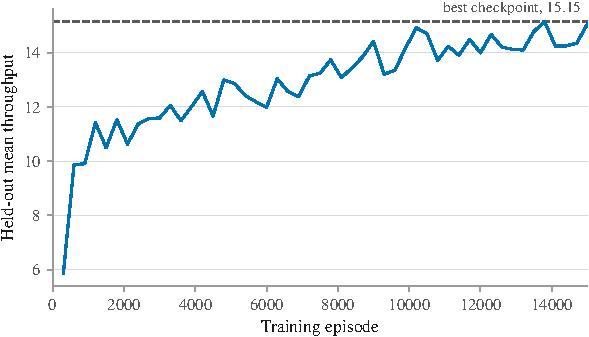
\includegraphics[width=4.60in]{images/report_inner_training.pdf}
  \caption{Held-out mean cumulative throughput of the inner PPO agent over
$15{,}000$ training episodes, evaluated every $300$ episodes. The dashed line marks
the best checkpoint, which is the one used for every result reported below.}
  \label{fig:job_scheduling_training}
\end{figure}

Figure~\ref{fig:policy_comparison} compares the mean throughput of every policy. Sia is evaluated in four configurations, obtained by crossing exclusive against shared GPUs and single-GPU against multi-GPU allocations: exclusive ($12.48 \pm 3.20$), exclusive with distribution ($12.99 \pm 3.97$), shared ($14.27 \pm 2.11$), and shared with distribution ($14.85 \pm 2.29$). Both axes behave as the cluster model predicts. Allowing GPU sharing raises Sia by $1.79$ without distribution and $1.86$ with it, because doubling the number of schedulable slots lets it serve every queued job rather than leaving the tail unscheduled. Allowing multi-GPU configurations raises it by a further $0.51$ (exclusive) and $0.58$ (shared): once the ILP has served every job, the capacity constraint in Eq.~\eqref{eq:sia} is what decides whether spare slots are worth spending on a second copy. This is a property of the global formulation, not of distribution per se---a greedy rule that duplicates whenever the immediate gain looks positive spends slots that later jobs need and \emph{loses} throughput.

\begin{figure}[H]
  \centering
  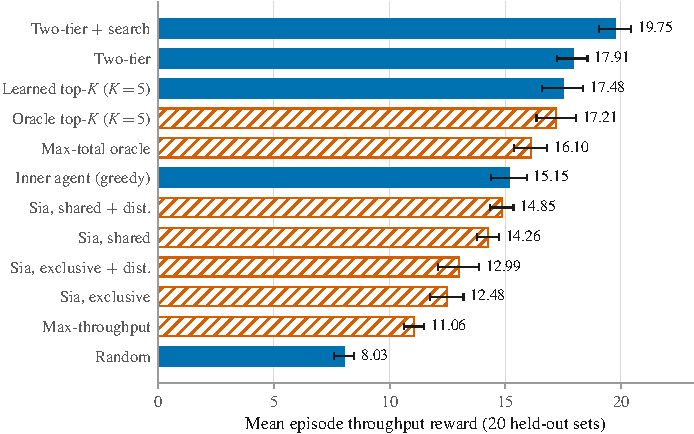
\includegraphics[width=4.60in]{images/report_policy_comparison.pdf}
  \caption{Mean cumulative throughput ($\pm$ standard error) of every evaluated
policy over the 20 held-out job sets. Hatched bars read exact throughputs at
decision time---the two oracles and the four Sia configurations---and are not
deployable schedulers.}
  \label{fig:policy_comparison}
\end{figure}

The inner agent, used greedily, reaches $15.15 \pm 3.48$, above every heuristic baseline---the best Sia variant ($14.85 \pm 2.29$), max-throughput ($11.06 \pm 1.99$) and random ($8.03 \pm 1.96$)---but below the max-total oracle ($16.10 \pm 3.20$). That the learned policy beats Sia while consuming only observable state, whereas Sia solves an ILP over the entire queue with exact throughput profiles, indicates that the gap is not one of search effort: Sia's normalized, fairness-shaped objective deliberately equalizes progress across jobs, which costs raw throughput on this metric.

The gap between the inner agent and the max-total oracle ($15.15$ vs.\ $16.10$) reflects \emph{where} each policy obtains its information, rather than a limitation of learning. At decision time the oracle re-scores \emph{every} candidate slot with the exact true throughput of the current job on that accelerator, including pair-specific co-location interference, and takes the maximum. The inner agent, by contrast, sees only the observable system state and takes the single most probable action under its policy. Because throughput depends only on the accelerator \emph{type} and the co-located job---all servers of the same type are interchangeable---many slots have identical true value, so the policy's distribution over the best slots is nearly uniform and a single argmax amounts to an arbitrary tie-break among near-optimal placements. The resulting per-decision errors are small but compound over the roughly 50 jobs of each job set. The deficit is therefore one of \emph{selection among near-ties}, not of missing information: re-scoring only the top-$K$ actions proposed by PPO and choosing the best among them ($K{=}3$ and $K{=}5$) already yields $16.61$ and $17.21$---\emph{above} the full-space oracle. That refinement is not deployable as stated, since it scores candidates with the true reward; Section~\ref{sec:results-oraclefree} shows it can be reproduced without one. The oracle resolves near-ties by a fixed enumeration order that ignores their impact on future jobs, whereas the learned prior breaks ties toward placements that leave the cluster in a better state for the jobs yet to arrive.
\subsection{Outer Agent and Joint Training}
\label{sec:outer}
The outer agent is trained for $10{,}000$ episodes on top of the inner agent,
under the two-phase regime of Section~\ref{sec:method}: the base placement is made
by a frozen copy of the inner policy, while a second copy is fine-tuned alongside
the outer agent to place the duplicates.

Figure~\ref{fig:subset_selector_training} shows both learning signals, evaluated on the held-out sets every $20$ episodes. The outer agent's own episode reward---the throughput its duplication decisions add---rises from $-2.13$ to roughly $+2.5$, crossing zero early in training: the agent starts by duplicating indiscriminately, which costs throughput, and learns to duplicate only where spare capacity makes it profitable. The total held-out throughput of the resulting two-tier schedule rises in step, from $13.02$ to $18.14$ at its best evaluation.

\begin{figure}[h]
  \centering
  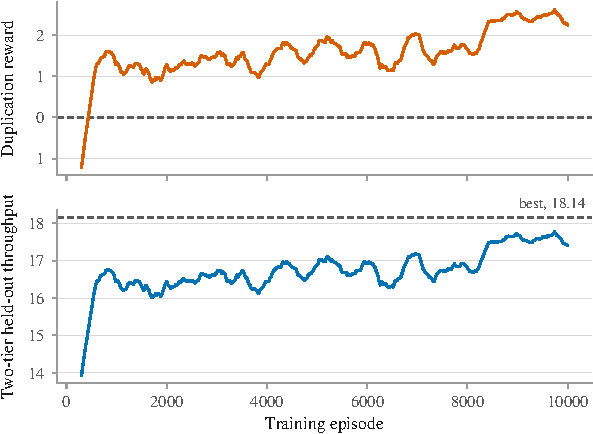
\includegraphics[width=4.60in]{images/report_outer_training.pdf}
  \caption{Joint training of the outer agent and the duplicate-placement policy
over $10{,}000$ episodes, evaluated every $20$ episodes and smoothed with a
$15$-point moving average. Top: reward from the duplication decisions alone,
which starts negative and crosses zero as the agent learns to duplicate only where
spare capacity makes it profitable. Bottom: total held-out throughput of the
complete two-tier schedule.}
  \label{fig:subset_selector_training}
\end{figure}

Re-evaluating the saved checkpoint end to end gives a mean cumulative throughput of $17.91 \pm 2.92$ on the held-out sets---an $18\%$ improvement over the inner agent alone ($15.15$), and above both the max-total oracle ($16.10$) and the strongest heuristic baseline, Sia with shared GPUs and distribution ($14.85 \pm 2.29$). It beats the oracle on $13$ of the $20$ held-out sets (Figure~\ref{fig:two_tier_per_set}). These results show that the outer agent's duplication decisions provide substantial throughput beyond what the placement agent can reach alone, and that freezing the base placement is enough to attribute that gain to the duplication tier.


\begin{figure}[H]
  \centering
  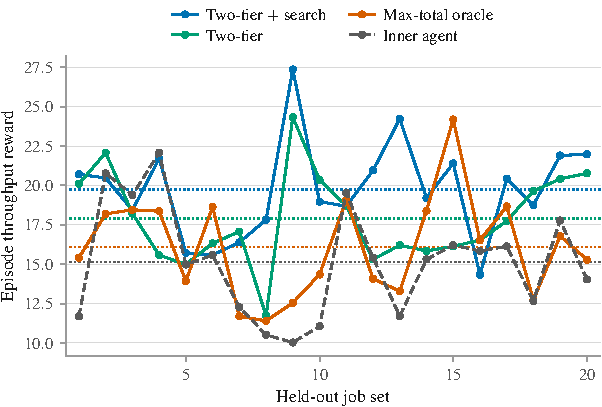
\includegraphics[width=4.60in]{images/report_two_tier_per_set.pdf}
  \caption{Per-set cumulative throughput across the 20 held-out job sets; dotted
lines mark the means. The two-tier system beats the max-total oracle on 13 of the
20 sets, and adding the oracle-free search raises it further on most of them.}
  \label{fig:two_tier_per_set}
\end{figure}

\subsection{The Oracle-Free Search Matches the Oracle-Assisted One}
\label{sec:results-oraclefree}

\begin{figure}[t]
\centering
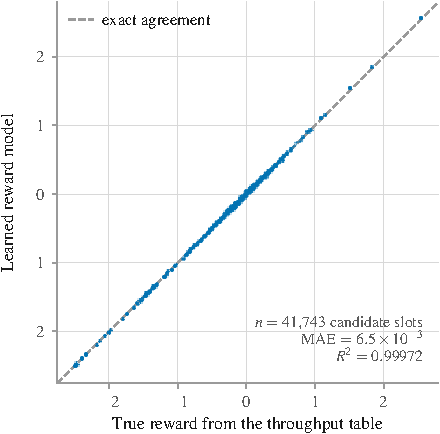
\includegraphics[width=3.50in]{images/report_reward_model.pdf}
\caption{The learned reward model against the oracle quantity it replaces, on
every feasible slot of greedy rollouts over the $20$ test sets. The throughput
tables are read here only to produce the horizontal axis; the model sees none of
it, and was fitted on randomly generated job sets.}
\label{fig:reward-model}
\end{figure}

Figure~\ref{fig:reward-model} shows the learned prediction against the true reward
for every feasible slot along greedy rollouts on the test sets. Over $41{,}743$
candidate slots the model attains $R^2 = 0.99972$ and a mean absolute error of
$6.5 \times 10^{-3}$ in reward units. On a validation split of its own training
distribution it agrees with the oracle's arg\,max on $98.3\%$ of decisions, at a
mean regret of $4.5 \times 10^{-5}$ per decision---roughly four orders of magnitude
below the scale of the rewards being compared.

\begin{table}[t]
\centering
\small
\caption{Mean $\pm$ standard deviation over the $20$ test sets, with paired
statistics against the oracle-free search. Italicised rows read exact throughputs
at decision time and are upper bounds, not deployable schedulers.}
\label{tab:main}
\begin{tabular}{lcrr}
\toprule
Policy & Test (20 sets) & $\Delta$ & paired $t$ \\
\midrule
Two-tier $+$ search (both phases)   & $\mathbf{19.76 \pm 3.08}$ & $+2.27$ & $+1.90$ \\
Two-tier $+$ search (primary only)  & $19.24 \pm 2.93$ & $+1.75$ & $+1.61$ \\
Two-tier                            & $17.91 \pm 2.92$ & $+0.42$ & $+0.38$ \\
Learned top-$K$ ($K{=}5$)           & $17.48 \pm 4.00$ & --- & --- \\
\textit{Oracle top-$K$ ($K{=}5$)}   & $17.21 \pm 3.84$ & $-0.28$ & $-2.06$ \\
Learned top-$K$ ($K{=}3$)           & $16.65 \pm 3.19$ & $-0.83$ & --- \\
\textit{Oracle top-$K$ ($K{=}3$)}   & $16.61 \pm 3.18$ & $-0.87$ & --- \\
\textit{Max-total oracle}           & $16.10 \pm 3.20$ & $-1.38$ & $-4.70$ \\
Inner agent (greedy)                & $15.15 \pm 3.48$ & $-2.33$ & $-3.91$ \\
\textit{Sia, shared $+$ distribution} & $14.85 \pm 2.29$ & $-2.64$ & --- \\
\bottomrule
\end{tabular}
\end{table}

Table~\ref{tab:main} gives the comparison. The oracle-free search reaches
$17.48 \pm 4.00$, reproducing the oracle-assisted refinement it replaces
($17.21$) while reading no throughput data at decision time, and beating the
max-total oracle by $+1.38$ (paired $t = 4.70$) and the inner agent alone by
$+2.33$ ($t = 3.91$). At $K{=}3$ the two versions are likewise level ($16.65$
against $16.61$). \emph{Reproducing} the oracle-assisted result without an oracle
is the claim this work supports; the $+0.28$ by which the learned search edges
ahead at $K{=}5$ is within the noise of a $20$-set comparison and we do not read
anything into it.

\subsection{Composing the Search with the Duplication Tier}
\label{sec:composition}

The search and the duplication agent are orthogonal: one improves \emph{where each
copy goes}, the other decides \emph{how many copies there are}. We therefore leave
the outer agent exactly as trained---it still decides whether each job is
duplicated---and replace only the placement step, which the two-tier system
performs twice per duplicated job.

\paragraph{Which placements the search performs.}
The scheduler places jobs with two different networks: the frozen primary policy for the
initial placement, and the fine-tuned secondary policy for duplicates
(Section~\ref{sec:method}). The search can replace either or both:

\begin{center}
\small
\begin{tabular}{lccc}
\toprule
 & initial placement & duplicate placement & Test (20 sets) \\
\midrule
Two-tier                       & primary, $\arg\max$ & secondary, $\arg\max$ & $17.91 \pm 2.92$ \\
Two-tier $+$ search (primary)  & \textbf{search}     & secondary, $\arg\max$ & $19.24 \pm 2.93$ \\
Two-tier $+$ search (both)     & \textbf{search}     & \textbf{search}       & $\mathbf{19.76 \pm 3.08}$ \\
\bottomrule
\end{tabular}
\end{center}

\noindent Replacing both placements gives $19.76 \pm 3.08$, which is $+1.85$ over
the two-tier baseline (paired $t = 2.73$, better on $13$ of the $20$ sets) and
$+2.27$ over the search alone. Using the search for the duplicates as well as the
initial placements adds $+0.52$ over using it for the initial placements only. It
also schedules with fewer duplicates ($6.1$ versus $7.5$ per episode): better
placement makes duplication less necessary.

\paragraph{The secondary policy becomes redundant.}
In the configuration above, both phases search over the \emph{primary} policy, so
the fine-tuned secondary network is bypassed rather than re-ranked. Searching the
duplicates over the secondary policy instead gives $19.78 \pm 2.89$, a difference
of $+0.03$ (paired $t = 0.13$). Which policy proposes the candidate slots is
therefore immaterial once the search selects among them---the fine-tuning that
Section~\ref{sec:outer} credits for part of the two-tier gain buys nothing that the
search does not already supply.

\paragraph{The duplicate score is an approximation.}
The initial phase is exact: no duplicates exist while it runs, so $\kappa$ fully
determines every candidate's reward. Placing a \emph{duplicate} additionally pays
$-d(s)\,(T_{\text{orig}} + T_{\text{dup}})$, and $T_{\text{orig}}$---the throughput
of the copy already running---is not a function of $\kappa$. The search therefore
ranks duplicate slots by an expression missing one term. It still helps, but this
is the one place in this work where the score is knowingly incomplete. In a real
deployment $T_{\text{orig}}$ is measurable on the running copy and should be
supplied; inside the simulator, reading it would mean querying the throughput
table.

\subsection{Ablations}
\label{sec:ablation}

\begin{figure}[t]
\centering
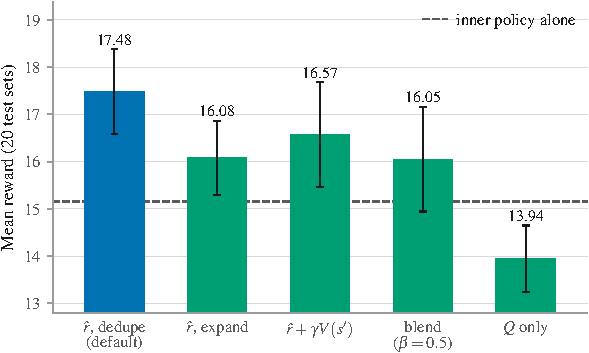
\includegraphics[width=4.60in]{images/report_ablation.pdf}
\caption{How the candidate set is built and what scores it, on the $20$ test
sets. Error bars are one standard error. The dashed line is the inner policy used
without any search. The winning configuration was selected on validation, not
here.}
\label{fig:ablation}
\end{figure}

Figure~\ref{fig:ablation} reports two findings that cut against the design
intuition, and we state them as results rather than footnotes.

\paragraph{Canonicalisation is a latency tool, not a quality tool.}
Used to \emph{deduplicate} a fixed top-$K$ list it is free: identical decisions,
$55\%$ fewer scorings, confirmed over $150$ decisions by an equivalence check.
Used to \emph{expand} the list into $K$ distinct classes, it reaches further down
the policy's ranking and scores $16.08$ against $17.48$. With a myopic score, a
wider candidate set simply makes the scheduler greedier; the policy's probability
ordering is itself a long-horizon signal, and widening the set discards it.

\paragraph{The learned long-horizon heads do not pay off at this scale.}
Every variant that consults them scores below the myopic one: $16.57$ for
$\hat r + \gamma V(s')$, $16.05$ for the blend, and $13.94$ for $Q$ alone---below
even the bare policy. Validation orders them identically, so the choice of the
myopic score was made there and merely confirmed here. The reason is a signal-to-noise mismatch. The value head's
validation MAE is ${\approx}0.48$ and the $Q$-head's TD loss plateaus at
${\approx}0.10$, while the reward differences between candidate slots are
${\sim}0.01$--$0.3$. The long-horizon term injects noise one to two orders of
magnitude larger than the signal it is meant to refine. The components are
implemented, trained and evaluated; the shipped default is myopic.


\subsection{Learning the Reward Model Online}
\label{sec:online-reward}

\begin{figure}[t]
\centering
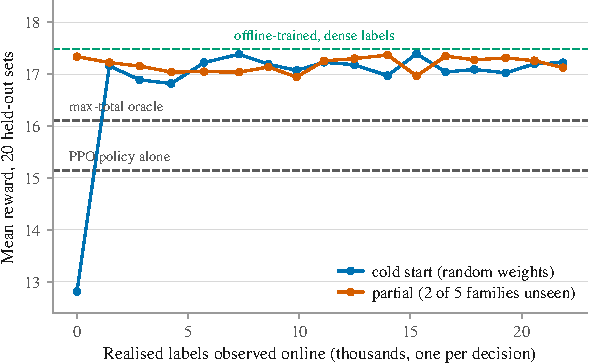
\includegraphics[width=4.60in]{images/report_online_reward_model.pdf}
\caption{Bootstrapping the reward model on live traffic with one label per
decision. The policy is frozen throughout, so the curve isolates the reward model.
The oracle top-$K$ reference ($17.21$) is omitted because it coincides with the
curves. Deployment stream: randomly generated job sets. Test: the $20$ held-out
sets, greedy, never learned from.}
\label{fig:online-reward}
\end{figure}

\textbf{A cold start costs about $1{,}500$ labels.} From random weights the search
scores $12.82$---below the bare policy, as expected when the candidate ranking is
noise. After $1{,}461$ realised labels, roughly $25$ episodes, it reaches $17.16$,
already past the max-total oracle ($16.10$); by $7{,}295$ labels it is at $17.38$,
level with the offline fit ($17.48$), and it plateaus there
(Figure~\ref{fig:online-reward}). The bootstrap is cheap for the same structural
reason the model is small: one shared function of $18$ inputs, so every decision
teaches it something that transfers to every slot.

\textbf{The search bounds the damage a bad model can do.} The partial model, which
never saw ResNet-50 or Transformer, scores $17.33$ \emph{before any online
update}---almost the full model's $17.48$. This is not generalisation. Measured
directly on held-out states, its error on the unseen families is $0.3300$ MAE
against $0.0052$ for the full model, $63\times$ worse, and $8.7\times$ worse than
its own error on the families it did see. What rescues the end-to-end score is the
candidate set: the top-$K$ are the policy's own best guesses, which are already
good placements, so mispricing among them costs little.

The practical reading is that \textbf{the policy sets the quality floor and the
reward model sets the ceiling}. The worst case measured---a random model, which
picks roughly uniformly among the policy's top five---is $12.82$, and a roughly
right model captures most of the available gain. For a component intended to be
deployed before it is fully trained, that is the failure mode one wants.

\subsection{Online Deployment and Decision Latency}
\label{sec:latency}

A key advantage of the learned schedulers over the max-total oracle is that they are directly usable as online policies. At decision time, the inner and outer agents consume only the observable system state---per-slot GPU occupancy, the current job's model type and batch size, and statistics of the remaining queue---and select an action with a single forward pass through their networks. Crucially, no throughput table is queried when choosing an action; throughput estimates appear only in the offline training reward and in the evaluation metric. The measurements below put every decision path on a common cluster state; all of them are far below the seconds-scale inter-arrival times of training jobs in a GPU cluster.

In contrast, the max-total oracle is an offline upper bound rather than a deployable scheduler. Each of its decisions re-evaluates every candidate slot using the exact true throughput of each job on each accelerator type, including pair-specific co-location interference. Such perfect, real-time profiling is precisely the information that is expensive or unavailable in production clusters, which is what motivates learning a scheduling policy from observations in the first place. The inner agent alone therefore lags the oracle slightly ($15.15$ vs.\ $16.10$), but the complete two-tier system \emph{surpasses} it ($17.91$ vs.\ $16.10$; Figure~\ref{fig:two_tier_per_set}). Two effects explain this. First, the oracle is \emph{myopic}: it greedily maximizes only the immediate total throughput of the current placement and, when several slots tie at the optimum, resolves the tie by a fixed enumeration order, without considering how the choice shapes the cluster for future jobs. The learned policies are instead trained to maximize cumulative return over an entire job set, so their tie-breaking favours placements that leave resources well-positioned for the jobs yet to arrive. Second, the outer agent's duplication decisions \emph{enlarge} the action space beyond what any single-placement policy---learned or not---can reach: placing a copy of a job on an underutilized accelerator, or on an accelerator that co-locates favourably with it, converts idle capacity into additional throughput. The oracle never duplicates, so its $16.10$ is an upper bound for the \emph{single-copy} scheduling problem; the two-tier system solves a strictly larger problem and exceeds that bound using only observable state and millisecond-scale decisions.




\begin{figure}[t]
\centering
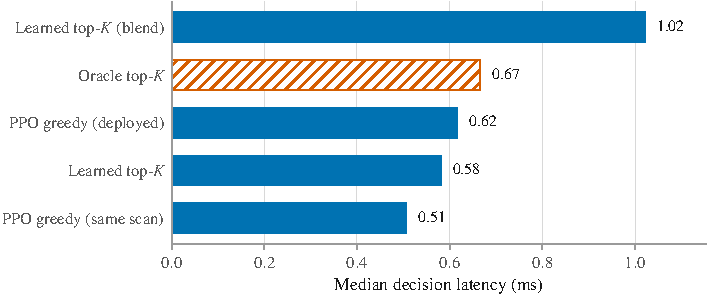
\includegraphics[width=4.60in]{images/report_latency.pdf}
\caption{Median latency of a full placement decision, measured on the same
half-full cluster state (eager fp32, one CPU thread, $400$ timed decisions after
warm-up). The hatched bar reads exact throughputs.}
\label{fig:latency}
\end{figure}

All five placement paths sit within a factor of two of each other
(Figure~\ref{fig:latency}). The oracle-free search costs $0.58$~ms, against
$0.50$~ms for a greedy decision built from the same feasibility scan: the search
itself adds $+0.08$~ms, or $15\%$. Two of its components are negligible---
canonicalising all $45$ slots costs $0.043$~ms and the delta next-state
construction $0.013$~ms---and the blended rule, which builds $K$ next
states and evaluates two additional networks, is the only path past a millisecond.
The inner forward pass alone takes $0.11$~ms and the outer duplication decision
$0.11$~ms. All are negligible against the seconds-scale inter-arrival times of
training jobs in a GPU cluster.

\textbf{Latency is not the argument for replacing the oracle, and we want to be
explicit about that.} The oracle top-$K$ runs in $0.66$~ms, only $14\%$ slower than
the learned search, because its true-reward evaluation is a handful of dictionary
lookups. An earlier version of this measurement reported the oracle at $4.59$~ms
and the deployed greedy actor at $1.16$~ms; both were dominated by an
$O(J \cdot S \cdot A)$ feasibility scan that every policy in the codebase shared.
Once that scan is vectorised in the one place feasibility is defined, the apparent
gap disappears. The case for the learned model rests on availability, not speed:
the oracle cannot be evaluated online at any latency, because the co-location it
prices has not happened yet.

\subsection{Continual Learning under Job-Mix Drift}
\label{sec:drift}

\begin{figure}[t]
\centering
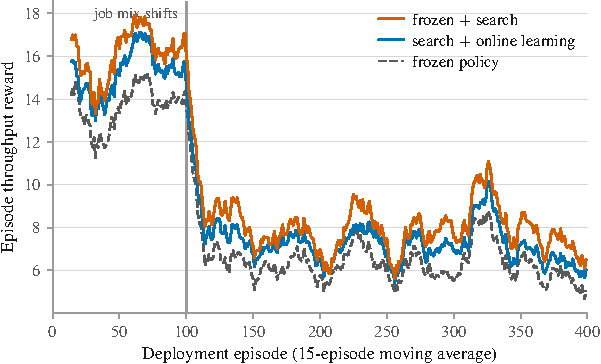
\includegraphics[width=4.60in]{images/report_drift.pdf}
\caption{A $400$-episode deployment stream whose job mix shifts at episode $100$
toward heavier models and larger batch sizes. All arms are served the identical
stream, so the comparison is paired.}
\label{fig:drift}
\end{figure}

\begin{table}[t]
\centering
\small
\caption{Post-shift results (episodes $100$--$400$). The policy-only probe measures
the deployed policy alone---greedy, no search---on a fixed probe set from the
current mix, separating what the policy learned from what the search contributes
and from the cost of exploring.}
\label{tab:online}
\begin{tabular}{lccc}
\toprule
 & Frozen & Frozen $+$ search & Search $+$ online learning \\
\midrule
Realised deployment return        & $6.25$ & $\mathbf{7.85}$ & $7.14$ \\
Policy-only probe (mean)          & $6.45$ & $6.45$ & $6.79$ $(+5.2\%)$ \\
Held-out sets (the \emph{old} mix) & $\mathbf{15.15}$ & --- & $14.19$ \\
\bottomrule
\end{tabular}
\end{table}

\begin{figure}[t]
\centering
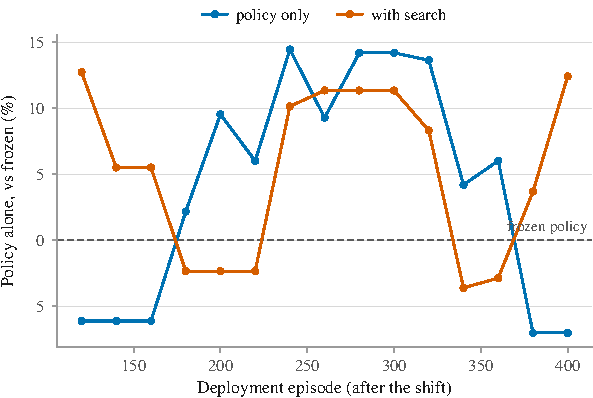
\includegraphics[width=4.60in]{images/report_probe.pdf}
\caption{The deployed policy measured alone---greedy, without the search---on a
fixed probe set from the drifted mix, relative to the frozen policy on the same
sets. The oscillation is the promotion gate: shadow evaluations on eight job sets
have limited statistical power, so regressions occasionally pass.}
\label{fig:probe}
\end{figure}

Figure~\ref{fig:drift} and Table~\ref{tab:online} give the drift experiment. The
headline is that \textbf{the search, not the learning, absorbs the drift}: with
frozen weights throughout, it lifts post-shift throughput from $6.25$ to $7.85$
($+25.6\%$). The learned reward model generalises over slot features---job type,
accelerator, co-located job---rather than over the job mix, so it stays accurate
when the mix changes.

Continual learning on top is a net negative over this horizon ($7.14$ versus
$7.85$). The policy it builds does improve: Figure~\ref{fig:probe} shows the
policy-only probe climbing to $+14\%$ against the frozen policy before falling
back. But roughly $10\%$ of steps spent exploring instead of searching costs more
than the policy gains within $300$ episodes, and adapting to the new mix costs
performance on the old one ($15.15 \rightarrow 14.19$ on the held-out sets), which
is ordinary catastrophic forgetting.

Decomposing the regression on the old mix separates the two learned pieces:

\begin{center}
\small
\begin{tabular}{llc}
\toprule
Policy & Reward model & Held-out mean \\
\midrule
frozen  & frozen  & $\mathbf{17.48}$ \\
frozen  & online-updated & $17.26$ \\
online-updated & frozen & $15.82$ \\
online-updated & online-updated & $15.95$ \\
\bottomrule
\end{tabular}
\end{center}

\noindent The reward model survives online updating---despite seeing one label per
decision instead of $45$, it costs only $-0.22$, and its mean regret on the old mix
is in fact lower than the offline model's ($2.7 \times 10^{-4}$ versus
$5.0 \times 10^{-4}$). The $-1.66$ comes from the policy. The practical reading is
to update the heads continuously and gate policy updates far more conservatively
than the defaults used here. The gate itself behaves as designed---$18$ of $40$
candidates promoted with $2$ rollbacks in the policy-only run, $15$ of $40$ with
$4$ rollbacks with the search---and its statistical power is the binding constraint
on adaptation speed: doubling the monitor set from $8$ to $16$ job sets raises the
probe gain from $+4.1\%$ to $+7.2\%$ and simultaneously deepens forgetting
($14.74 \rightarrow 13.90$).



\section{Discussion}

Two aspects of these results deserve separate treatment: what our evaluation
procedure does and does not establish, and why two of the components we built did
not earn their place.

\subsection{What the Selection Procedure Costs}
\label{sec:selection}

Two of the systems compared here have their checkpoints chosen by a score on the
test sets: the inner agent keeps the checkpoint with the best held-out evaluation,
and the outer agent keeps the best of ${\sim}500$ evaluations taken every $20$
episodes across $10{,}000$ episodes. That is selection
on the reporting set, and it inflates those two numbers by an amount we cannot
measure from the test sets alone.

Scoring the same systems on $40$ validation sets---randomly generated, used for no
training and no reporting---indicates that the inflation is real and unequal. The
two-tier system leads the oracle-free search by $+0.42$ on the test sets but
trails it by $-0.56$ on validation, a reversal consistent with its $500$-draw
selection procedure; the search's own margin over the max-total oracle, by
contrast, holds at $+1.04$ ($t = 5.60$). We therefore selected every configuration
introduced in this paper on validation (Section~\ref{sec:protocol}) and report the
two-tier numbers as they stand, noting that the comparison between the two-tier
system and the search is the one that should not be read as settled.


\subsection{Why Two Components Did Not Pay Off}

The learned long-horizon heads and the continual policy updates were both built on
sound reasoning and both lost. It is worth saying why, because the two failures
have the same shape.

In each case a learned quantity was asked to resolve a distinction finer than its
own error. The value head estimates returns to within ${\approx}0.48$ and the
$Q$-head's temporal-difference loss settles near $0.10$, while the reward
differences separating candidate slots are $0.01$--$0.3$; consulting them
therefore injects noise one to two orders of magnitude larger than the signal it
is meant to refine (Section~\ref{sec:ablation}). The continual policy updates fail
in the same way at the level of the deployment loop: a promotion gate judging
candidates on eight job sets cannot reliably detect the improvements the updates
produce, so regressions pass and gains are discarded, and the exploration needed
to generate the updates costs more throughput than they return
(Section~\ref{sec:drift}).

The contrast with the components that did work is instructive. The reward model
succeeds because it predicts a quantity that is a deterministic function of an
observable, low-dimensional statistic---so its error is small relative to the
distinctions it must make---and canonicalisation succeeds because it is exact by
construction rather than estimated at all. Where a scheduling decision hinges on a
quantity that can be identified exactly, identifying it beats learning it; where it
hinges on a long-horizon estimate, the policy's own ranking, trained on full
episode returns, is a more reliable carrier of that information than a separately
learned value function.

\section{Limitations}
\label{sec:limitations}

\paragraph{``Oracle-free'' describes decision time, not training.}
\label{sec:limitations-profiling}
The offline reward model is supervised by the throughput tables and is, in effect,
a learned compression of them. That is the intended reading---a deployment profiles
its own cluster offline and then schedules without querying---but it means the
contribution is the removal of a runtime dependency, not of the information
itself. Section~\ref{sec:online-reward} removes the offline profiling too: a cold
start recovers the same performance from about $1{,}500$ realised labels. It also
settles the extrapolation question in the negative---the model does \emph{not}
transfer to job families it never saw ($63\times$ worse prediction error)---and
shows why that matters less than expected, since the policy's candidate set bounds
the cost of mispricing.

\paragraph{The duplicate-placement score is incomplete.}
As noted in Section~\ref{sec:composition}, $T_{\text{orig}}$ is missing from the
feature vector. The measured effect is positive, but the component is an
approximation where the rest of the method is exact.

\paragraph{Single seed.}
The learned heads were fitted once, with one seed, and the two PPO agents were
each trained once. The evaluation protocol controls for selection over
\emph{configurations}, not over training runs; the paired statistics quantify
variation across job sets only.

\paragraph{Static queue.}
Each episode schedules a fixed job set with no arrivals, completions or
preemption. Extending the formulation to a continuously arriving queue is the most
significant piece of future work.

\paragraph{Simulated cluster.}
Everything is measured inside the Gavel-derived simulator. Latency figures come
from real CPU timings, but the throughput model, the interference model and the
distribution discounts are all simulator assumptions.



\section{Conclusion}

We presented a two-tier reinforcement learning scheduler for heterogeneous
GPU clusters, and then removed the one assumption that kept its strongest variant
from being deployable.

The two-tier system reaches a mean cumulative throughput of $17.91 \pm 2.92$ on the
held-out sets, above the inner agent alone ($15.15$), the max-total greedy oracle
($16.10$), and the strongest Sia configuration ($14.85 \pm 2.29$). Against Sia the
learned scheduler wins despite seeing strictly less: Sia solves an integer program
over the entire queue using exact throughput profiles, whereas our agents act
online from observable state. Against the max-total oracle the gain comes from the
duplication tier, which reaches placements no single-copy policy can express.

Diagnosing the inner agent's remaining deficit as one of tie-breaking led to a
top-$K$ refinement that surpasses the oracle---but scores candidates with the true
reward, and so is not a scheduler. Making it deployable turned out to need a
structural observation rather than a larger model: the placement reward has an
exact $18$-dimensional sufficient statistic readable from the scheduler's own
bookkeeping, which simultaneously collapses reward-equivalent candidates and
reduces the learning problem to a small shared function that predicts the oracle's
quantity to $R^2 = 0.99972$. The resulting search reproduces the oracle-assisted
refinement on the held-out sets, costs $0.58$~ms per decision with no throughput
lookup---verified by a guard that makes the tables raise on access---and composed
with the duplication tier gives the strongest configuration we measure, $19.76$. Bootstrapped from random weights on live traffic, it
recovers that performance after about $1{,}500$ realised rewards.

Two components did not earn their place, and we report them as such. The learned
long-horizon heads are dominated by their own estimation error at this problem
scale, and full continual online learning costs more in exploration than it returns
within the horizon tested, while degrading performance on the original job mix. The
more useful finding is the one that made them unnecessary: because the learned
reward model generalises over slot features rather than over the job mix, the
frozen search already absorbs a distribution shift severe enough to halve
throughput.

Finally, the evaluation protocol proved as consequential as the method. Two of the
systems compared here have their checkpoints chosen by a score on the reporting
set, and a validation stream that nothing was selected on shows the effect is
large enough to reverse one of the comparisons. Every configuration introduced in
this paper is therefore selected on validation and reported on the held-out sets,
and we recommend the same separation for any future number from this line of
work.

Future work could extend the formulation to online scheduling with dynamic job
arrivals, explore transfer across cluster configurations, and investigate job
preemption and elastic scaling.


\section*{Reproducibility}

All results are produced by a single evaluation entry point that scores every
policy on the same $20$ held-out job sets and reports the difference from the
committed values, so any drift is visible immediately. The three exactness claims
in Section~\ref{sec:oraclefree}---that canonicalisation is reward-preserving, that
the delta-built next observation matches the environment, and that the search
never reads the throughput tables while deciding---are implemented as executable
checks rather than assertions in prose, and each is run as part of the standard
verification pass. Every figure is regenerated from the stored measurement data by
one script, so no figure can diverge from the numbers it depicts.

\section*{Acknowledgments}


\bibliographystyle{unsrt}
\bibliography{references}

\end{document}
